\chapter{Problem Solving Paradigms}
\label{chap:ProblemSolvingParadigms}

\section{Overview and Motivation}

\large{\upshape{As commonly known or almost problem solving paradigms that is known, four problem solving paradigms. So in this chapter, we will discuss  commonly used namely like: Complete Search (a.k.a Brute Force), Divide and Conquer, the Greedy approach, and Dynamic Programming.}}
\\
\newline
\textbf{{\Large{So, we can assume the Backtrackig function as following:}}}


\begin{lstlisting}{c++}
        void backtrack(state) {
        if (hit end state or invalid state) // we need terminating or
            return; // pruning condition to avoid cycling and to speed up search
        for each neighbor of this state // try all permutation
             backtrack(neighbor);
        }
\end{lstlisting}

\newpage


\section{8-Queen Problem (Recursive Complete Search -Backtracking-)}
\label{8-Queen}

\href{https://vj.z180.cn/a1d3d6853584bb15ac7da3eeee0977ca?v=1575822738}{\color{red}{\textbf {UVa 750}}}\textbf{ - 8 Queens Chess Problem}

\begin{figure}[h]
    \centering
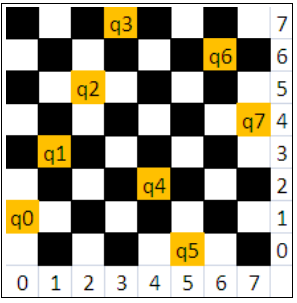
\includegraphics[width=6cm, height=6cm]{8-queen-problem.png}
 \caption{\textbf{8-Queens problem competitive programming 3, p.74}}
    \label{fig:8-queen-problem}
\end{figure}

Abridged problem statement: In chess (with an $8$ × $8$ board), it is possible to place eight queens on the board such that no two queens attack each other. Determine all such possible arrangements given the position of one of the queens (i.e. coordinate ($a$, $b$) must contain a queen). Output the possibilities in $lexicographical$ (sorted) order.
\\

\hspace{7mm}The most naive solution is to enumerate all combinations of 8 different cells out of the
8 × 8 = 64 possible cells in a chess board and see if the 8 queens can be placed at these positions without conflicts. However, there are $_6_4C_8$ $\approx$ $4B$ such possibilities—this idea is not even worth trying.
\\
 
\hspace{7mm}A better but still naive solution is to realize that each queen can only occupy one column, so we can put exactly one queen in each column. There are only $8^8$ $\approx$ $17M$ possibilities now,
down from $4B$. This is still a ‘borderline’-passing solution for this problem. If we write a Complete Search like this, we are likely to receive the Time Limit Exceeded (TLE) verdict especially if there are multiple test cases. We can still apply the few more easy optimizations described below to further reduce the search space.

\hspace{7mm}We know that no two queens can share the same column or the
same row. Using this, we can further simplify the original problem
to the problem of finding valid permutations of 8! row positions.
The value of \lstinline|row[i]| describes the row position of the queen in
column i. Example: \lstinline|row = {1, 3, 5, 7, 2, 0, 6, 4}| as in Figure\ref{fig:8-queen-problem} is one of the solutions for this problem;  \lstinline|row[0] = 1| implies that the queen in column 0 is placed in row 1, and so on (the index starts from 0 in this example). Modeled this way, the search space goes down from $8^8$ $\approx$ $17M$ to $8!$ $\approx$ $40K$  This solution is already fast enough, but we can still do more.
\\

\hspace{7mm}We also know that no two queens can share any of the two diagonal lines. Let queen A be at \lstinline|(i, j)| and queen B be at \lstinline|(k, l)|. They attack each other if \lstinline|abs(i-k) == abs(j-l)|. This formula means that the vertical and horizontal distances between these two queens are equal, i.e. queen A and B lie on one of each other’s two diagonal lines.
\\

\hspace{7mm}A recursive backtracking solution places the queens one by one in columns 0 to 7, observing all the constraints above. Finally, if a candidate solution is found, check if at least one of the queens satisfies the input constraints, i.e. \lstinline|row[b] == a|. This sub (i.e. lower than) $O(n!)$ solution will obtain an AC verdict.
\\

\begin{lstlisting}{c++}
        /* 8 Queens Chess Problem */
        #include<bits/stdc++.h>
        
        using namespace std;
        
        int row[8], TC, a, b, lineCounter; //ok to use global variables
        
        bool place(int r, int c) {
          for (int prev = 0; prev < c; prev++) //check previously placed queens
            if (row[prev] == r || (abs(row[prev] - r) == abs(prev - c)))
              return false;//share same row or same diagonal -> infeasible
          return true; }
        
        void backtrack(int c) {
          if (c == 8 && row[b] == a) {// candidate sol, (a, b) has 1 queen
            cout << ++lineCounter << "      " << row[0] + 1;
            for (int j = 1; j < 8; j++)cout << row[j] + 1;
            cout << endl; }
          for (int r = 0; r < 8; r++) // try all possible row
            if (place(r, c)) {//if can place a queen at this col and row
              row[c] = r; backtrack(c + 1); // put this queen here and recurse
        }   }
        
        int main() {
          cni >> TC;
          while (TC--) {
            cin >> a >> b; a--; b--;//switch to 0-based indexing
            memset(row, 0, sizeof row); lineCounter = 0;
            cout << SOLN <<         << COLUMN << endl;
            cout << # <<      << 1 2 3 4 5 6 7 8 << endl << endl;
            backtrack(0); //generate all possible 8! candidate solutions
            if (TC)cout << endl;
        } }   

\end{lstlisting}

\clearpage


\section{N-queen Problem (More Challenging Backtracking)}
\label{n-Queen}

\href{https://vj.z180.cn/7e4e8d92abc27cb470b49794bd31bb31?v=1575831964}{\color{red}{\textbf {UVa 11195}}}\textbf{ - N Queens Chess Problem}

\begin{figure}[h]
    \centering
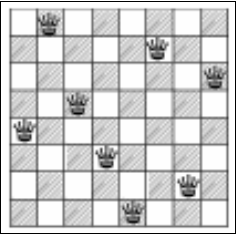
\includegraphics[width=6cm, height=6cm]{n-queen-problem.png}
 \caption{\textbf{N-Queens problem UVa 11195}}
    \label{fig:n-queen-problem}
\end{figure}

Abridged problem statement: Given an $n$ × $n$ chessboard ($3$ $<$ $n$ $<$ $15$) where some of the cells are bad (queens cannot be placed on those bad cells), how many ways can you place $n$ queens in the chessboard so that no two queens attack each other? Note: Bad cells cannot be used to block queens’ attack.

\hspace{7mm}The recursive backtracking code that we have presented above is not fast enough for $n = 14$ and no bad cells, the worst possible test case for this problem. The $sub-O(n!)$ solution presented earlier is still OK for $n = 8$ but not for $n$ = 14. We have to do better. The major issue with the previous $n$-queens code is that it is quite slow when checking whether the position of a new queen is valid since we compare the new queen’s position with the previous \lstinline|c-1| queens’ positions (see function \lstinline|bool place(int r, int c)|).

\hspace{7mm}Initially all n rows (rw), 2 × n − 1 left diagonals (ld), and 2 × n − 1 right diagonals (rd) are unused (these three bitsets are all set to false). When a queen is placed at cell (r, c), we flag rw[r] = true to disallow this row from being used again. Furthermore, all (a, b) where abs(r - a) = abs(c - b) also cannot be used anymore. There are two possibilities after removing the abs function: r-c=a-b and r+c=a+b. Note that r+c and r-c represent indices for the two diagonal axes. As r-c can be negative, we add an offset of n-1 to both sides of the equation so that r-c+n-1=a-b+n-1. If a queen is placed on cell (r, c), we flag ld[r - c + n - 1] = true and rd[r + c] = true to disallow these two diagonals from being used again. With these additional data structures and the additional problem-specific constraint in UVa 11195 (board[r][c] cannot be a bad cell), we can extend our code to become:

\begin{lstlisting}{c++}
        void backtrack(int c) {
        if (c == n) { ans++; return; } // a solution
        for (int r = 0; r < n; r++) // try all possible row
            if (board[r][c] != ’*’ && !rw[r] && !ld[r - c + n - 1] && !rd[r + c]) {
            rw[r] = ld[r - c + n - 1] = rd[r + c] = true; // flag off
            backtrack(c + 1);
            rw[r] = ld[r - c + n - 1] = rd[r + c] = false; // restore
        } }
\end{lstlisting}

\newpage
%\section{8-queen \& N-queen Problem Using Bitmask}

\section{Dynamic Programming}\label{sec:dp}
\subsection{Overview and Motivation}
Dynamic Programming (from now on abbreviated as DP) is perhaps the most challenging problem-solving technique among the four paradigms. The key skills that you have to develop in order to master DP are the abilities to determine the problem states and to determine the relationships or transitions between current problems and their sub-problems. We have used these skills earlier in recursive backtracking (see Section \ref{n-Queen} \& \ref{8-Queen}). In fact, DP problems with small input size constraints may already be solvable with recursive backtracking. DP is primarily used to solve optimization problems and counting problems. If you encounter a problem that says “minimize this” or “maximize that” or “count the ways to do that”, then there is a (high) chance that it is a DP problem. Most DP problems ask for the optimal/total value and not the optimal solution itself, which often makes the problem easier to solve by removing the need to backtrack and produce the solution. However, some harder DP problems also require the optimal solution to be returned in some fashion. We will continually refine our understanding of Dynamic Programming in this section.

\subsection{Knapsack Problem (0/1 Knapsack)}
Also called subset sum. So the problem is, he is a thief, who has a bag. This bag has a specific weight. He will enter a house and will steal things from this house. Everything has a specific weight and value he knows it. For example, he can take a gold ring. Although it is very light, it has a high benefit or a high value. And he can steal T.V. Although it has a low value, it has a high weight. The problem asks you, which items he can take, such that, these the weight of items fit in this bag + benefit of these items have a high cost as possible? 

\hspace{7mm}This problem is called.  This problem is also called 0/1 knapsack. It means that this item will be picked or it will be left -pick or leave-.
\newpage
\begin{figure}[h]
    \centering
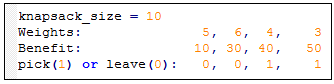
\includegraphics[width=14cm, height=3cm]{knapsack-example-1.png}
 \caption{\textbf{Knapsack Example 1}}
    \label{fig:knapsack-example-1}
\end{figure}
\\
\hspace{7mm}A cursory look at the example data tells us that the max value that we could accommodate with the limit of max weight of 10 is 50 + 40 = 90 with a weight of 7. 

\begin{figure}[h]
    \centering
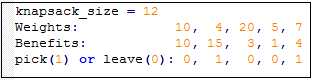
\includegraphics[width=14cm, height=3cm]{knapsack-example-2.png}
 \caption{\textbf{Knapsack Example 2}}
    \label{fig:knapsack-example-2}
\end{figure}
\\
\hspace{7mm}Also, a cursory look at the example data tells us that the max value that we could accommodate with the limit of max weight of 10 is 15 + 4 = 19 with a weight of 11.
\subsubsection{Recursion Implementation}
\begin{lstlisting}{c++}
        #include <bits/stdc++.h>
        #define INF INT_MIN
        
        using namespace std;
        
        struct item{
        	int weight;
        	int benefit;
        };
        
        int noOfItems;
        vector<item> items;
        int knapsack01(int index, int reminder) {
        	if (reminder < 0)return -INF;
        	if (reminder == 0 || index == noOfItems)return 0;
        	int Choice1 = knapsack01(index + 1, reminder);///I don't take the item, so i will go the next one i + 1. And the weight will still unchanged in the bag,
        	int Choice2 = knapsack01(index + 1, reminder - items[index].weight) + items[index].benefit;///After we take the item, i will go to the one after me, and i will remove the weight that i take it so far.
        	return max(Choice1, Choice2);
        }
        
        int main() {
        	ios_base::sync_with_stdio(0), cin.tie(0), cout.tie(0);
        	int tests; cin >> tests;
        	while (tests--) {
        		int weights;
        		cin >> noOfItems >> weights;
        		items = vector<item>(noOfItems);
        		for (int i = 0; i < noOfItems; i++)cin >> items[i].weight;
        		for (int i = 0; i < noOfItems; i++)cin >> items[i].benefit;
        		cout << knapsack01(0, weights) << endl;
        	}
        }
\end{lstlisting}

\subsubsection{DP (Top Down Approach) Implementation}
\begin{lstlisting}{c++}
        #include <bits/stdc++.h>
        #define INF INT_MIN
        
        using namespace std;
        
        struct item{
        	int weight;
        	int benefit;
        };
        
        const int MAX = 1001;
        int mem[MAX][MAX];
        int noOfItems;
        vector<item> items;
        
        int knapsack01(int index, int reminder) {
        	if (reminder < 0)return -INF;
            if (reminder == 0 || index == noOfItems)return 0;
        	int& bestChoice = mem[index][reminder];
        	if (~bestChoice)return bestChoice; ///as the same as, if (bestChoice != -1)
        	bestChoice = knapsack01(index + 1, reminder);///I don't take the item, so i will go the next one i + 1. And the weight will still unchanged in the bag,
        	bestChoice = max(bestChoice, knapsack01(index + 1, reminder - items[index].weight) + items[index].benefit);///After we take the item, i will go to the one after me, and i will remove the weight that i take it so far.
        	return bestChoice;
        }
        
        int main() {
        	ios_base::sync_with_stdio(0), cin.tie(0), cout.tie(0);///To fast input and output
        	int tests; cin >> tests;
        	while (tests--){
                int weights;
                cin >> noOfItems >> weights;
                items = vector<item>(noOfItems);
                for (int i = 0; i < noOfItems; i++)cin >> items[i].weight;
                for (int i = 0; i < noOfItems; i++)cin >> items[i].benefit;
                cout << knapsack01(0, weights) << endl;
            }
        }
\end{lstlisting}

\newpage

\subsection{Traveling Sales Man Problem (TSP)}
Problem: Given $n$ cities and their pairwise distances in the form of a matrix dist of size $n$ × $n$, compute the cost of making a tour18 that starts from any city $s$, goes through all the other $n$ − 1 cities exactly once, and finally returns to the starting city $s$.

\begin{figure}[h]
    \centering
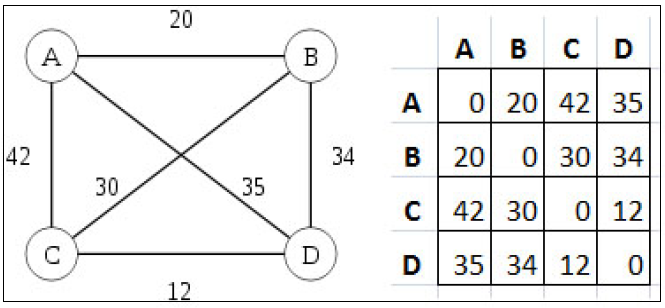
\includegraphics[width=14cm, height=7cm]{TSP.png}
 \caption{Complete Graph To Visualize TSP, \textbf{CP 3 book}}
    \label{fig:TSP}
\end{figure}

\hspace{7mm}Example: The graph shown in Figure \ref{TSP} has $n$ = 4 cities. Therefore, we have 4! = 24 possible tours (permutations of 4 cities). One of the minimum tours is \textbf{A-B-C-D-A} with a cost of \textbf{20+30+12+35 = 97} (notice that there can be more than one optimal solution).

\hspace{7mm}A ‘brute force’ TSP solution (either iterative or recursive) that tries all $O((n - 1)!)$ possible tours (fixing the first city to vertex A in order to take advantage of symmetry as the graph is undirected) is only effective when $n$ is at most $12$ as 11 $!$$\approx$ 40$M$. When $n$$>$12, such brute force solutions will
get a TLE in \textbf{Online Judges}. However, if there are multipl test cases, the limit for such ‘brute force’ TSP solution is probably just $n$ = 11.

\hspace{7mm}We can utilize DP for TSP since the computation of sub-tours is clearly overlapping, e.g. the tour \textbf{A - B - C - (n - 3)} other cities that finally return to A clearly overlaps the tour \textbf{A - C - B - the same (n - 3)} other cities that also return to A. If we can avoid re-computing the lengths of such \textbf{sub-tours}, we can save a lot of computation time. However, a distinct state in TSP depends on two parameters: The last \textbf{city/vertex} visited pos and something that we may have not seen before—a subset of visited cities.

\hspace{7mm}There are many ways to represent a set. However, since we are going to pass this set
information around as a parameter of a recursive function (if using top-down DP), the representation we use must be lightweight and efficient! In Section \ref{sec:dp}. If we have $n$ cities, we use a binary integer of length n. If bit i is ‘1’ (on), we say that item (city) $i$ is inside the set (it has been visited) and item $i$ is not inside the set (and has not been visited) if the bit is instead $‘0’$ (off). For example: mask= 1810 = 100102 implies that items (cities) {1, 4} are in19 the set (and have been visited). Recall that to check if bit $i$ is on or off, we can use \lstinline|{mask & (1 << i)}|. To set bit $i$, we can use \lstinline{mask |= (1 << i)} .

\begin{lstlisting}{c++}
        const int INF = 1e9;
        int BottomUp(vector<vector<int> > dist) { //Distance between city(i,j);
            int n = dist.size();
            int lim = 1 << n; //It means, 2 to the power n
            int dp[lim][n];
            memset(dp, INF, sizeof(dp));
            for (int i = 0; i < n; i++) {
                dp[1 << i][i] = 0;    // base case of visiting just 1 city
            }
            for (int mask = 0; mask < lim; mask++) {
                for (int last = 0; last < n; last++) {
                    if (mask & (1 << last) == 0) { // Didn't visit last.
                        continue;
                    }
                    for (int curr = 0; curr < n; curr++) {
                        if (mask & (1 << curr) == 0) { // Didn't visit current
                            continue;
                        }
                        int otherMask = mask ^ (1 << curr);
                        dp[mask][curr] = min(dp[mask][curr], dp[otherMask][last] + dist[last][curr]);
                    }
                }
            }
            int ans = INF;
            for (int i = 0; i < n; i++) {
                ans = min(ans, dp[lim - 1][i]);
            }
            return ans;
        }
        
        int memo[][];
        int TopDown(int pos,int mask){
          if (mask == (1 << V) - 1)
        			return cost[pos][0];
          if (memo[pos][mask]!=-1) {
            return memo[pos][mask];
          }
        		int min = INF;
        		for (int nxt = 0 ; nxt < V ; ++nxt)
        			if (nxt != pos && (mask & (1 << nxt)) == 0)
        				min = Math.min(min, cost[pos][nxt] + TopDown(nxt, mask | (1 << nxt)));
        		return memo[pos][mask] = min;
        	}
        }

\end{lstlisting}
